\documentclass[11pt]{article}
\usepackage[T1]{fontenc}
\usepackage{amsmath}
\usepackage{amsfonts, amssymb}
\usepackage{xcolor}
\usepackage{tikz}

\begin{document}

On the left is a colored $q$-Boson model (where color 1 is red and color 2 is blue). On the right is its associated colored line ensemble $\bm{L} = \big( \bm{L}^{(1)}, \bm{L}^{(2)} \big)$ (where $\bm{L}^{(1)}$ is purple, and $\bm{L}^{(2)}$ is blue).

\begin{figure}[h]
    \centering
    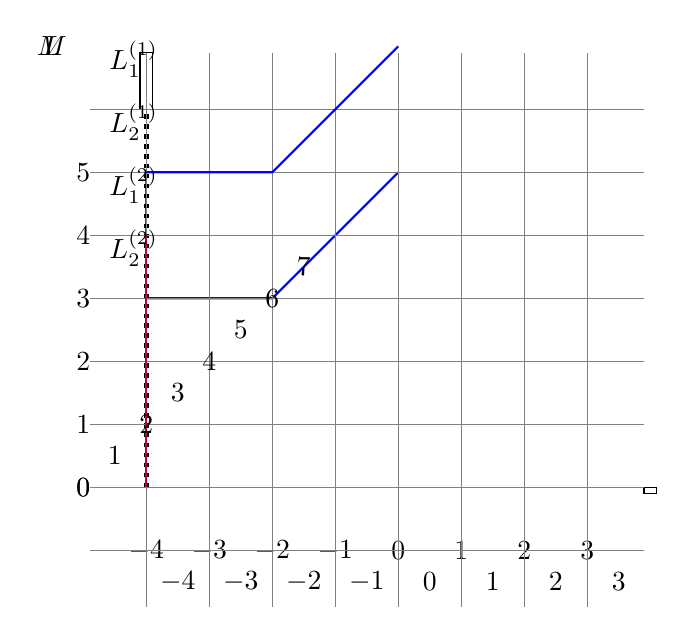
\begin{tikzpicture}[scale=0.8]
        % Left side
        \draw[step=1cm,gray,thin] (-3.9,-1.9) grid (3.9,6.9);
        \draw[thick,red] (-4,0) -- (-4,5); % Color 1 path
        \draw[thick,blue] (-4,3) -- (-2,3) -- (0,5); % Color 2 path
        \draw[ultra thick,dotted] (-4,0) -- (-4,6);
        \filldraw[fill=white] (-3.9,6) rectangle (-4.1,6.9);
        \filldraw[fill=white] (3.9,-.1) rectangle (4.1,0);

        \foreach \i in {-4,...,3}
            {\node at (\i,-1) {$\i$};}   
        \foreach \j in {0,...,5}
            {\node at (-5,\j) {$\j$};} 
        \node at (-5.5,7) {$M$};
    
        % Right side
        \draw[step=1cm,gray,thin] (-4.9,-1.9) grid (3.9,6.9);
        
        \draw[thick,purple] (-4,0) -- (-4,4); % Line L^{(1)}
        \draw[thick,blue] (-4,5) -- (-2,5) -- (0,7); % Line L^{(2)}
        
        \foreach \i in {-4,...,3}
            {\node at (\i+0.5,-1.5) {$\i$};}   
        \foreach \j in {0,...,7}
            {\node at (-5+\j/2,\j/2) {$\j$};} 
        
        \node at (-5.5,7) {$\bm{L}$};
        \node at (-4.2,6.8) {$L_{1}^{(1)}$};
        \node at (-4.2,5.8) {$L_{2}^{(1)}$};
        \node at (-4.2,4.8) {$L_{1}^{(2)}$};
        \node at (-4.2,3.8) {$L_{2}^{(2)}$};
        
    \end{tikzpicture}
\end{figure}

\end{document}